
%(BEGIN_QUESTION)
% Copyright 2011, Tony R. Kuphaldt, released under the Creative Commons Attribution License (v 1.0)
% This means you may do almost anything with this work of mine, so long as you give me proper credit

This turbine speed-control system does not appear to be regulating turbine speed properly.  The PV as shown on the controller is substantially below SP, and has been for quite a while.  You happen to notice that the controller output reads 100\% on the faceplate:

$$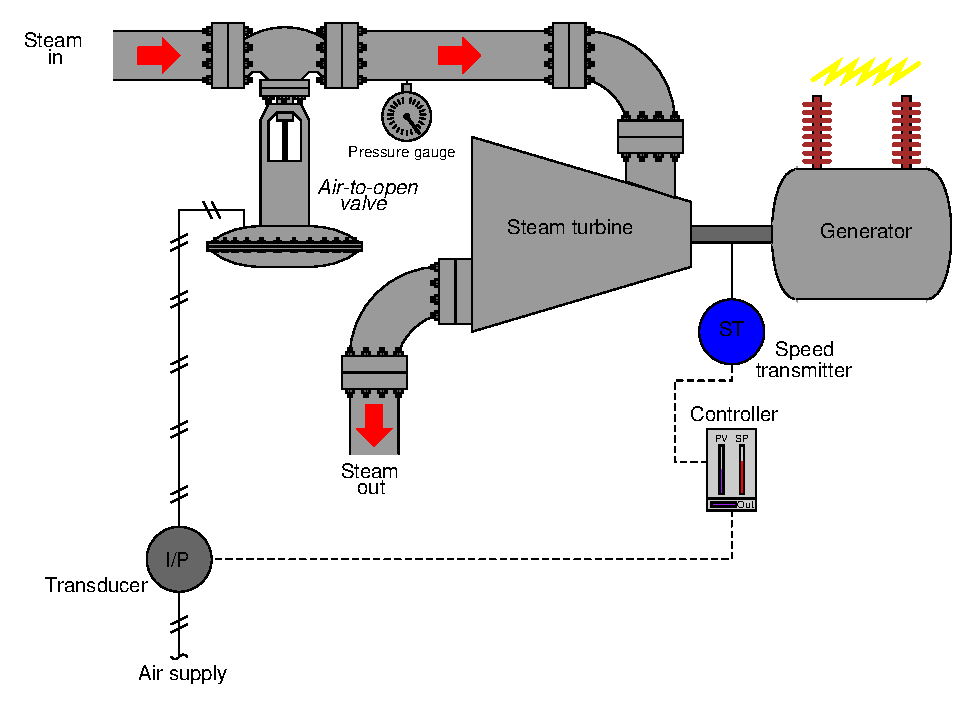
\includegraphics[width=15.5cm]{i00441x01.eps}$$

Your first test is to measure loop current in the control valve (I/P) circuit.  There, your multimeter registers 20.03 milliamps.

\vskip 10pt

Identify the likelihood of each specified fault for this control system.  Consider each fault one at a time (i.e. no coincidental faults), determining whether or not each fault could independently account for {\it all} measurements and symptoms in this circuit.

% No blank lines allowed between lines of an \halign structure!
% I use comments (%) instead, so that TeX doesn't choke.

$$\vbox{\offinterlineskip
\halign{\strut
\vrule \quad\hfil # \ \hfil & 
\vrule \quad\hfil # \ \hfil & 
\vrule \quad\hfil # \ \hfil \vrule \cr
\noalign{\hrule}
%
% First row
{\bf Fault} & {\bf Possible} & {\bf Impossible} \cr
%
\noalign{\hrule}
%
% Another row
ST out of calibration (outputting wrong current) &  &  \cr
%
\noalign{\hrule}
%
% Another row
SIC input out of calibration (not interpreting signal properly) &  &  \cr
%
\noalign{\hrule}
%
% Another row
SIC output out of calibration (not sending correct mA signal to I/P) &  &  \cr
%
\noalign{\hrule}
%
% Another row
Pressure gauge out of calibration (not displaying pressure properly) &  &  \cr
%
\noalign{\hrule}
%
% Another row
I/P out of calibration (not outputting correct pressure) &  &  \cr
%
\noalign{\hrule}
%
% Another row
Control valve is oversized &  &  \cr
%
\noalign{\hrule}
%
% Another row
Control valve is undersized &  &  \cr
%
\noalign{\hrule}
%
% Another row
SIC is poorly tuned (not making good control ``decisions'') &  &  \cr
%
\noalign{\hrule}
%
% Another row
Instrument air supply not at full pressure &  &  \cr
%
\noalign{\hrule}
} % End of \halign 
}$$ % End of \vbox

\underbar{file i00441}
%(END_QUESTION)





%(BEGIN_ANSWER)

This is a graded question -- no answers or hints given!

%(END_ANSWER)





%(BEGIN_NOTES)

The fact that the controller's output is saturated high as its PV is well below SP tells us the controller is trying as hard as it can to get the PV up to SP.  Thus, the controller is making ``good'' decisions and its PID algorithm is not at fault.  This is all we can tell from an inspection of the controller's faceplate.  After this, we need to check for real-world correspondence with the PV and Output values.

\vskip 10pt

Our first test reveals the controller is actually putting out the right amount of current for the 100\% Output display.  This tells us there is good correspondence between the controller's Output display and its real-world output signal.  However, we still do not know if the control valve is actually wide-open, which means it's possible for there to be a problem with the I/P, the instrument air supply, or the valve itself.

\vskip 10pt

Another possibility -- one that is frequently missed by students reading this problem -- is that a problem could exist on the measurement side of the loop.  We have no diagnostic data at this point to tell us whether or not the low PV value shown on the controller faceplate agrees with the actual turbine speed.  This means it's possible that we have some sort of calibration error on the system's measurement side: either with the speed transmitter or with the controller's PV signal input.  In other words, for all we know now it's possible that the true turbine speed is actually {\it above} setpoint, but that we're not seeing the true speed at the controller due to some fault in the measurement components.

% No blank lines allowed between lines of an \halign structure!
% I use comments (%) instead, so that TeX doesn't choke.

$$\vbox{\offinterlineskip
\halign{\strut
\vrule \quad\hfil # \ \hfil & 
\vrule \quad\hfil # \ \hfil & 
\vrule \quad\hfil # \ \hfil \vrule \cr
\noalign{\hrule}
%
% First row
{\bf Fault} & {\bf Possible} & {\bf Impossible} \cr
%
\noalign{\hrule}
%
% Another row
ST out of calibration (outputting wrong current) & $\surd$ &  \cr
%
\noalign{\hrule}
%
% Another row
SIC input out of calibration (not interpreting signal properly) & $\surd$ &  \cr
%
\noalign{\hrule}
%
% Another row
SIC output out of calibration (not sending correct mA signal to I/P) &  & $\surd$ \cr
%
\noalign{\hrule}
%
% Another row
Pressure gauge out of calibration (not displaying pressure properly) &  & $\surd$ \cr
%
\noalign{\hrule}
%
% Another row
I/P out of calibration (not outputting correct pressure) & $\surd$ &  \cr
%
\noalign{\hrule}
%
% Another row
Control valve is oversized &  & $\surd$ \cr
%
\noalign{\hrule}
%
% Another row
Control valve is undersized & $\surd$ &  \cr
%
\noalign{\hrule}
%
% Another row
SIC is poorly tuned (not making good control ``decisions'') &  & $\surd$ \cr
%
\noalign{\hrule}
%
% Another row
Instrument air supply not at full pressure & $\surd$ &  \cr
%
\noalign{\hrule}
} % End of \halign 
}$$ % End of \vbox

%INDEX% Basics, control loop troubleshooting: determining cause of control problem
%INDEX% Process: steam turbine generator

%(END_NOTES)


